\section{Reinforcement learning}

Reinforcement Learning refers to a kind of Machine Learning method in which an agent learns to solve a given task by maximizing the received reward signal. Where the agent represents the reinforcement learning algorithm.\\


\begin{figure}[H]
  \centering
  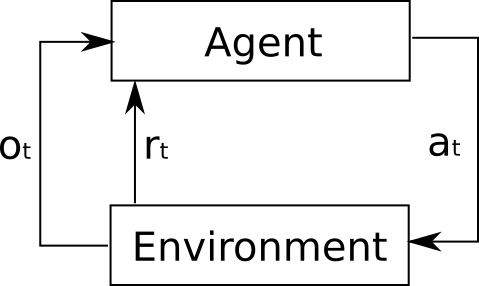
\includegraphics[width=300px]{Images/rl_agent.png} 
  \caption{Agent: reinforcement learning algorithm; Environment: object the agent is acting on; $a_t$ action the agent performance in the environment; $o_t$: observation (current state) of the environment the agent receives; $r_t$ reward signal the agent receives from the environment}
  \label{fig:reinforcement_learning}
\end{figure}


Figure \ref{fig:reinforcement_learning} shows the interaction of the agent with the environment where the environment refers to the object the agent is acting on. As initial state the agent receives the observation $o_t$ of the environment at time $t = 0$. The observation $o_t$ can be the complete state of the environment or just a subset of it.
%(For example when learning the movement of a roberter the observation could be the view from the robot onto the environment.)
The agent then, based on the observation $o_t$, perform an action $a_t$ in the environment, chosen from a set of possible actions (e.g. moving to the right or moving to the left). After performing the action $a_t$ the agent receives the new observation $o_{t+1}$ of the environment and also the reward signal $r_{t+1}$ which evaluates how good the chosen action was.
Based on the two new information the agent again choose an action $a_t$. The loop continuous until the environment sent a termination state.\\

%To maximize the received reward, the agent use the received reward signal to update it's action choosing function also called policy. The goal of the agent is to learn an optimal policy too maximize the received reward.\\

The goal of the agent is to maximize the received reward, which is done by learning an optimal action choosing function called policy using the received reward signal.
There exists different reinforcement learning algorithm which all follow the above described iterative learning algorithm, but differ in the update strategy for learning an optimal policy. In the following a short overview over different types of reinforcement learning algorithm will be  given.\\

\subsection{Q-learning}

Q-learning is a reinforcement learning algorithm which was introduced by Watkins \cite{QLearning} in 1989. 
For any finite markov decision processes, Q-learning finds a policy that maximized the expected total reward over all following steps, starting from the current state.
%Q-Learning is guarantee to converge to an optimal solution TODO ref.\\
To do so Q-Learning learns a Q-table, which contains for each state-action pair $(s, a)$ a Q-value which represents the expected future reward for taking the action $a$ in state $s$. 
By iteratively update the Q-value function with the Bellman Equation the Q-value function will converge to the optimal Q-value function \cite{QLearningProof}.\\

The Bellman equation 

%To calculate the Q-value function, the Bellman equation is used, which states that each state can be represented by the previouse state:\\

\begin{equation} \label{eq:bellman_eq1}
Q_{\pi} (s_t, a_t) =\mathbb{E}_{s_{t+1}} [r + \lambda Q_\pi(s_{t+1}, a_{t+1}) | s_t, a_t]
\end{equation}

states, that the Q-value for the state-action pair $(s_t, a_t)$ is equal to the expectation of the received reward $r$, of taking action $a$ in state $s$, plus the discounted future reward the agent will get by following the policy $\pi$ from the next state onwards, where $\lambda$ refers to the discount factor.\\

%By iteratively update the Q-value function with the Bellman Equation the Q-value function will converge to the optimal Q-value function and will learn to choose the optimal actions. \\


%\begin{equation}
%v(s) = \mathbb{E} [R_{t+1} + \lambda v(S_{t+1}) | S_t = s]
%\end{equation}

%$\mathbb{E}$ in the above equation refers to the expectation, while $\lambda$ refers to the discount factor. We can re-write it in the form of Q-value:


The optimal Q-value, denoted as $Q^* (s_t, a_t)$ can be expressed as:
\begin{equation} \label{eq:1}
Q^* (s_t, a_t) = \mathbb{E}_{s_{t+1}} [r + \lambda \max_{a'} Q^*(s_{t+1}, a_{t+1}) | s_t, a_t]
\end{equation}

After the agent has converged to the optimal policy $Q^* (s_t, a_t)$ it is able to to choose in each possible state the optimal action.\\

%The goal is to maximize the Q-value.

%To receive our goal to maximize the expected reward, we want to find a function which calculates the maximum expected future reward, for each action at each state. So when we in a certain state we can simple ask this function about the expected reward for each possible action we can take and choose the best one.

%Value based methods: where we learn a value function that will map each state action pair to a value. The action with the biggest value is the best action to take for each state.

%The base idear behind reinforcement learning is the Bellman Equation. By iteratively update the Q-value function the Q-value function will converge to the optimal Q-value function and will learn to choose the optimal actions. 

%Q-Learning is an off-policy, model-free RL algorithm based on the Bellman Equation:


\subsection{Value-based versus policy-based reinforcement learning methods}

Value-based methods are learning a value function which will map state-action pairs directly to values. The best action can then be found by taking for each state the action with the biggest value. 
An example of a value-based method is the in the previous section mentioned Q-learning method.
Policy-based methods, in contrast to value-based methods, optimize the policy directly without using of a value function.
The main problem of policy-based methods is to find a good score function to compute how good a policy is. An example of a policy-based method is reinforcement learning with policy gradient.

%Value based methods (Q-learning, Deep Q-learning): where we learn a value function that will map each state action pair to a value. Thanks to these methods, we find the best action to take for each state-the action with the biggest value. This works well when you have a finite set of actions.\\

%Policy based methods (REINFORCE with Policy Gradients): where we directly optimize the policy without using a value function. This is useful when the action space is continuous or stochastic. The main problem is finding a good score function to compute how good a policy is. We use total rewards of the episode.

\subsection{Model-free versus model-based reinforcement learning}

Model-free reinforcement learning maps observation of the environment directly to values or actions.
%Observations of the environment map directly to values or actions	

In contrast to this model-based reinforcement learning algorithm are using a model of the environment to simulate the dynamics of the environment. The model knows the transition probability $T(s_{t+1} | s_t, a_t)$ to the next state $s_{t+1}$ given the current state $s_t$ and the current action $a_t$. By taking this model into account adverse consequences of trial-and error can be avoid, also the performance of the agent can be increased by increasing the amount of internal simulations.
But there are some drawbacks. If the model is imperfect the performance of model-based agents suffers. Also it is not always possible to get an exact transition model or to get an transition model at all. In real world application it is often impossible to get a good enough transition model.\\




%For more information about reinforcement learning see TODO


\subsection{Deep Q network}

In the paper "Human-level control through deep reinforcement learning" Mnih et. al. \cite{dqn} introduce the first reinforcement learning algorithm which uses a neuronal network as a function approximation for the Q-value function. Reinforcement learning algorithm which are using a neuronal network as function approximation are also called deep reinforcement learning.\\
%Deep reinforcement learning means that the algorithm is using a neuronal network to learn the decission making function.

The approximated target values are:

\begin{equation} \label{eq:1}
y = r + \lambda \max_{a'} Q(s_{t+1}, a_{t+1}; \theta_i^-)
\end{equation}

The network parameters can than be optimized by minimizing the loss between the optimal target values and the approximated target value. Because the optimal target values are not know a second network with fixed weights $\theta^-$ is used. The loss function looks as follow:

\begin{equation} \label{eq:dqn_loss}
L_i(\theta_i) = \mathbb{E}_{s, a, r}[(\mathbb{E}_{s_{t+1}} [ y | s, a] - Q(s, a; \theta_i))^2]
\end{equation}

%The Q-value update function looks than as follow:
%\begin{equation}
%Q (s_t, a_t; \theta) = \mathbb{E}_{s_{t+1}} [r + \lambda \max_{a'} Q(s_{t+1}, a_{t+1}) | s_t, a_t; \theta^-]
%r_j + \gamma \max_{a'} Q(s{t+1}, a'; \theta^-)
%\end{equation}

For more details see the paper \cite{dqn}.\\



\subsection{Advantage-actor-critic}
\label{sec:a2c}

Mnih et al. introduce in the paper "Asynchronous Methods for Deep Reinforcement Learning" \cite{A3C} the deep reinforcement learning algorithm asynchronous advantage-actor-critic (A3C). Short after introduced A3C Mnih et. al. published a synchronous, deterministic variant of A3C called advantage-actor-critic (A2C) which gives equal performance.
A2C combines value-based and policy-based reinforcement learning and consist of two parts. A critic which measures how good a taken action is (value-based) and an actor which controls how the agent behaves (policy-based).\\
% an \textbf{actor} and a \textbf{critic} function, both are heads of a neuronal network.\\

The \textbf{actor} learns the policy function $\pi(a | s, \theta)$, probability of choosing action $a$ given state $s$, which is used to decide the best action $a$ given a specific state $s$.
The actor controls how the agent behaves.
$\theta$ are the learnable weights of the neural network. \\

The \textbf{critic} learns the value function $\mathnormal{V(s, w)}$, which measures how good a certain state $s$ is to be in. The value function $V$ is used to calculate the expected cumulative reward $Q(s, a)$ from following the policy $\pi$ from state $s$.

\begin{equation}
	Q(s, a) = r_{t+1} + \gamma V^\pi(s_{t+1})
\end{equation}

To update the policy function, the \textbf{Advantage function} is used which tells the improvement of a certain action compared to the average action taken at state $s$. 
In other words, it estimate the improvement of the true reward compared to the expected reward of the current state $s$ by using the temporal difference error:

\begin{equation}
	A(s, a) = Q(s, a) - V(s)
\end{equation}

The advantage function push up the probability of an action from a state $s$ if this action was better than the expected value.\\

\textbf{policy $\pi(a | s, \theta)$ loss}: 

\begin{equation}
	loss_\pi = - log (\pi_\theta(a | s)) * A
\end{equation}

\textbf{policy $\pi(a | s, \theta)$ gradient}:


\begin{equation}
	\nabla \theta = A \nabla_\theta log \pi_\theta (a | s)
\end{equation}
	
\textbf{value $V(s, w)$ loss}:

\begin{equation}
	loss_V = \sum(R - V(s))^2
\end{equation}


%messures how good a choosen actions is. 
%And which is used to calculate the expected cumulative reward from following the policy $\pi$ from state $s$.\\
%A critic is used for evaluating the policy function estimated by the actor according to the temporal difference (TD) error.

%Advantage function
%This function will tell us the improvement compared to the average the action taken at that state is. In other words, this function calculates the extra reward I get if I take this action. The extra reward is that beyond the expected value of that state.\\
%		Push up the probability of an action from a state $s$ if this action was better than the expected value
%A^{\pi_\theta} = Q^{\pi_\theta}(s, a) - V^{\pi_\theta}(s)		
		

